% Primary source: https://sites.engineering.ucsb.edu/~jbraw/mpc/
\documentclass[tikz,border=5pt]{standalone}
\usepackage[T1]{fontenc}
\usepackage{lmodern,amsmath,amssymb}
\usetikzlibrary{arrows.meta,calc,positioning,fit,backgrounds,shapes.geometric,matrix,decorations.pathreplacing,patterns}
\definecolor{ink}{gray}{0.08}
\definecolor{wash}{gray}{0.965}
\definecolor{soft}{gray}{0.45}
\tikzset{box/.style={draw=ink,line width=.65pt,fill=white,align=center,inner sep=4pt,outer sep=0pt,font=\small},flow/.style={draw=ink,line width=.65pt,-{Latex[length=1.8mm,width=1.3mm]},rounded corners=2pt},annotation/.style={font=\scriptsize,text=soft,align=center},groupbox/.style={draw=soft,dashed,line width=.45pt,fill=wash}}
\begin{document}
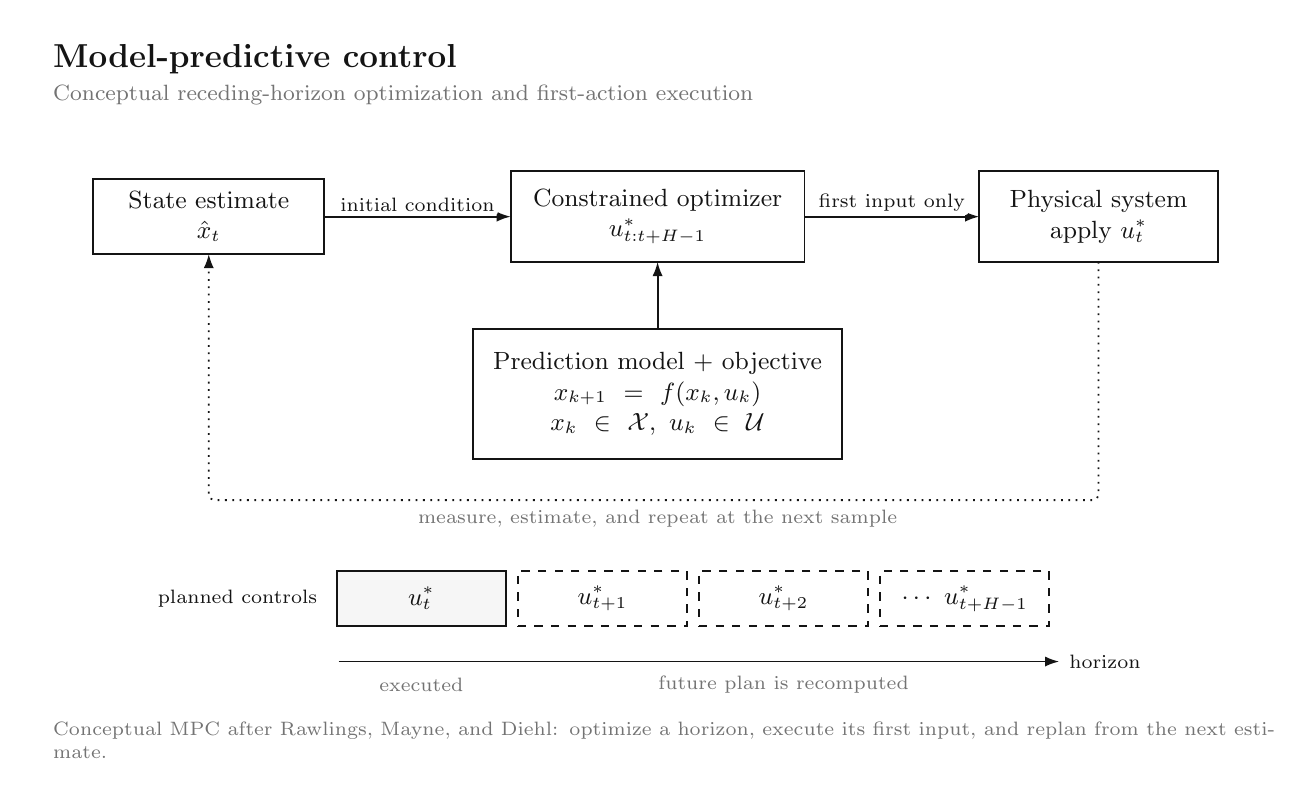
\begin{tikzpicture}[x=1cm,y=-1cm,font=\rmfamily,text=ink]

\path[use as bounding box] (0,0) rectangle (16,9.3);
\node[anchor=west,font=\large\bfseries] at (.2,.4) {Model-predictive control};
\node[anchor=west,font=\footnotesize,text=soft] at (.2,.85) {Conceptual receding-horizon optimization and first-action execution};
\begin{pgfonlayer}{background}
\end{pgfonlayer}
\node[box,minimum width=2.9cm,minimum height=0.95cm,text width=2.65cm] (estimate) at (2.3,2.4) {State estimate\\$\hat{x}_t$};
\node[box,minimum width=3.7cm,minimum height=1.15cm,text width=3.45cm] (opt) at (8.0,2.4) {Constrained optimizer\\$u^*_{t:t+H-1}$};
\node[box,minimum width=3.0cm,minimum height=1.15cm,text width=2.75cm] (plant) at (13.6,2.4) {Physical system\\apply $u_t^*$};
\node[box,minimum width=4.65cm,minimum height=1.65cm,text width=4.4cm] (model) at (8.0,4.65) {Prediction model + objective\\$x_{k+1}=f(x_k,u_k)$\\$x_k\in\mathcal{X},\ u_k\in\mathcal{U}$};
\begin{pgfonlayer}{background}
\draw[flow] (estimate.east) -- (opt.west) node[midway,above,fill=white,inner sep=1.5pt,font=\scriptsize] {initial condition};
\draw[flow] (opt.east) -- (plant.west) node[midway,above,fill=white,inner sep=1.5pt,font=\scriptsize] {first input only};
\draw[flow] (model.north) -- (opt.south);
\draw[flow,dotted] (plant.south) -- (13.6,6.0) -- (2.3,6.0) -- (estimate.south);
\end{pgfonlayer}
\node[annotation,text width=10.6cm] at (8.0,6.23) {measure, estimate, and repeat at the next sample};
\node[anchor=east,font=\scriptsize] at (3.8,7.25) {planned controls};
\node[box,fill=wash,minimum width=2.15cm,minimum height=.7cm] at (5.0,7.25) {$u_t^*$};
\node[box,fill=white,dashed,minimum width=2.15cm,minimum height=.7cm] at (7.3,7.25) {$u_{t+1}^*$};
\node[box,fill=white,dashed,minimum width=2.15cm,minimum height=.7cm] at (9.6,7.25) {$u_{t+2}^*$};
\node[box,fill=white,dashed,minimum width=2.15cm,minimum height=.7cm] at (11.9,7.25) {$\cdots\ u_{t+H-1}^*$};
\draw[flow] (3.95,8.05) -- (13.1,8.05) node[right,font=\scriptsize] {horizon};
\node[annotation] at (5.0,8.35) {executed};\node[annotation] at (9.6,8.35) {future plan is recomputed};
\node[anchor=west,align=left,font=\scriptsize,text=soft,text width=15.6cm] at (.2,9.05) {Conceptual MPC after Rawlings, Mayne, and Diehl: optimize a horizon, execute its first input, and replan from the next estimate.};
\end{tikzpicture}
\end{document}
